% Chapter 3

\chapter{\uppercase{System Design}}
\label{ch:design}
This chapter describes the design requirements, the architecture and the five modules,
following the Maya example through them.

\section{\uppercase{Design Requirements}}
We worked from a few rules. Original messages are saved exactly as sent \emph{before}
any extraction, which runs later as a queued job, so a failed model call can't lose a
conversation. A changed fact is a new version and the old value is kept with its validity
interval, never overwritten. Every fact links to an exact quote that is checked against the
original message. All data belongs to a namespace (e.g.\ \code{user:maya}) and whatever
we hand to a model or the agent has to fit a token budget. Models run locally on Ollama.
Duplicates, crashed workers and bad model output are handled with stored jobs, leases,
retries and validation, and Neo4j is only a copy that can be rebuilt from PostgreSQL.

\section{\uppercase{Overall Architecture}}
Figure~\ref{fig:architecture} shows the overall architecture. The client is the Pi coding agent.
Its memory client saves every message through the memory service and asks for recall
before answering. The memory service itself is a Rust application with API handlers and
asynchronous workers, and it depends on four other components.

PostgreSQL with pgvector is the main store, shared by M1 to M4. It holds the
evidence (sessions, episodes, events, chunks), the entities, assertions, sources and
vectors, and the job queue. Ollama runs the models: our fine-tuned worker model for
M2 (and reflection in M4), and a Qwen3 embedding model for vectors. Neo4j keeps a
graph copy of the assertions and entities, joined by \code{MENTIONS} and \code{SUPPORTS} edges.
M4 rechecks every graph hit against PostgreSQL before using it.  M5 runs offline (live chats are \emph{not} used as training data).

\begin{figure}[htbp]
\centering
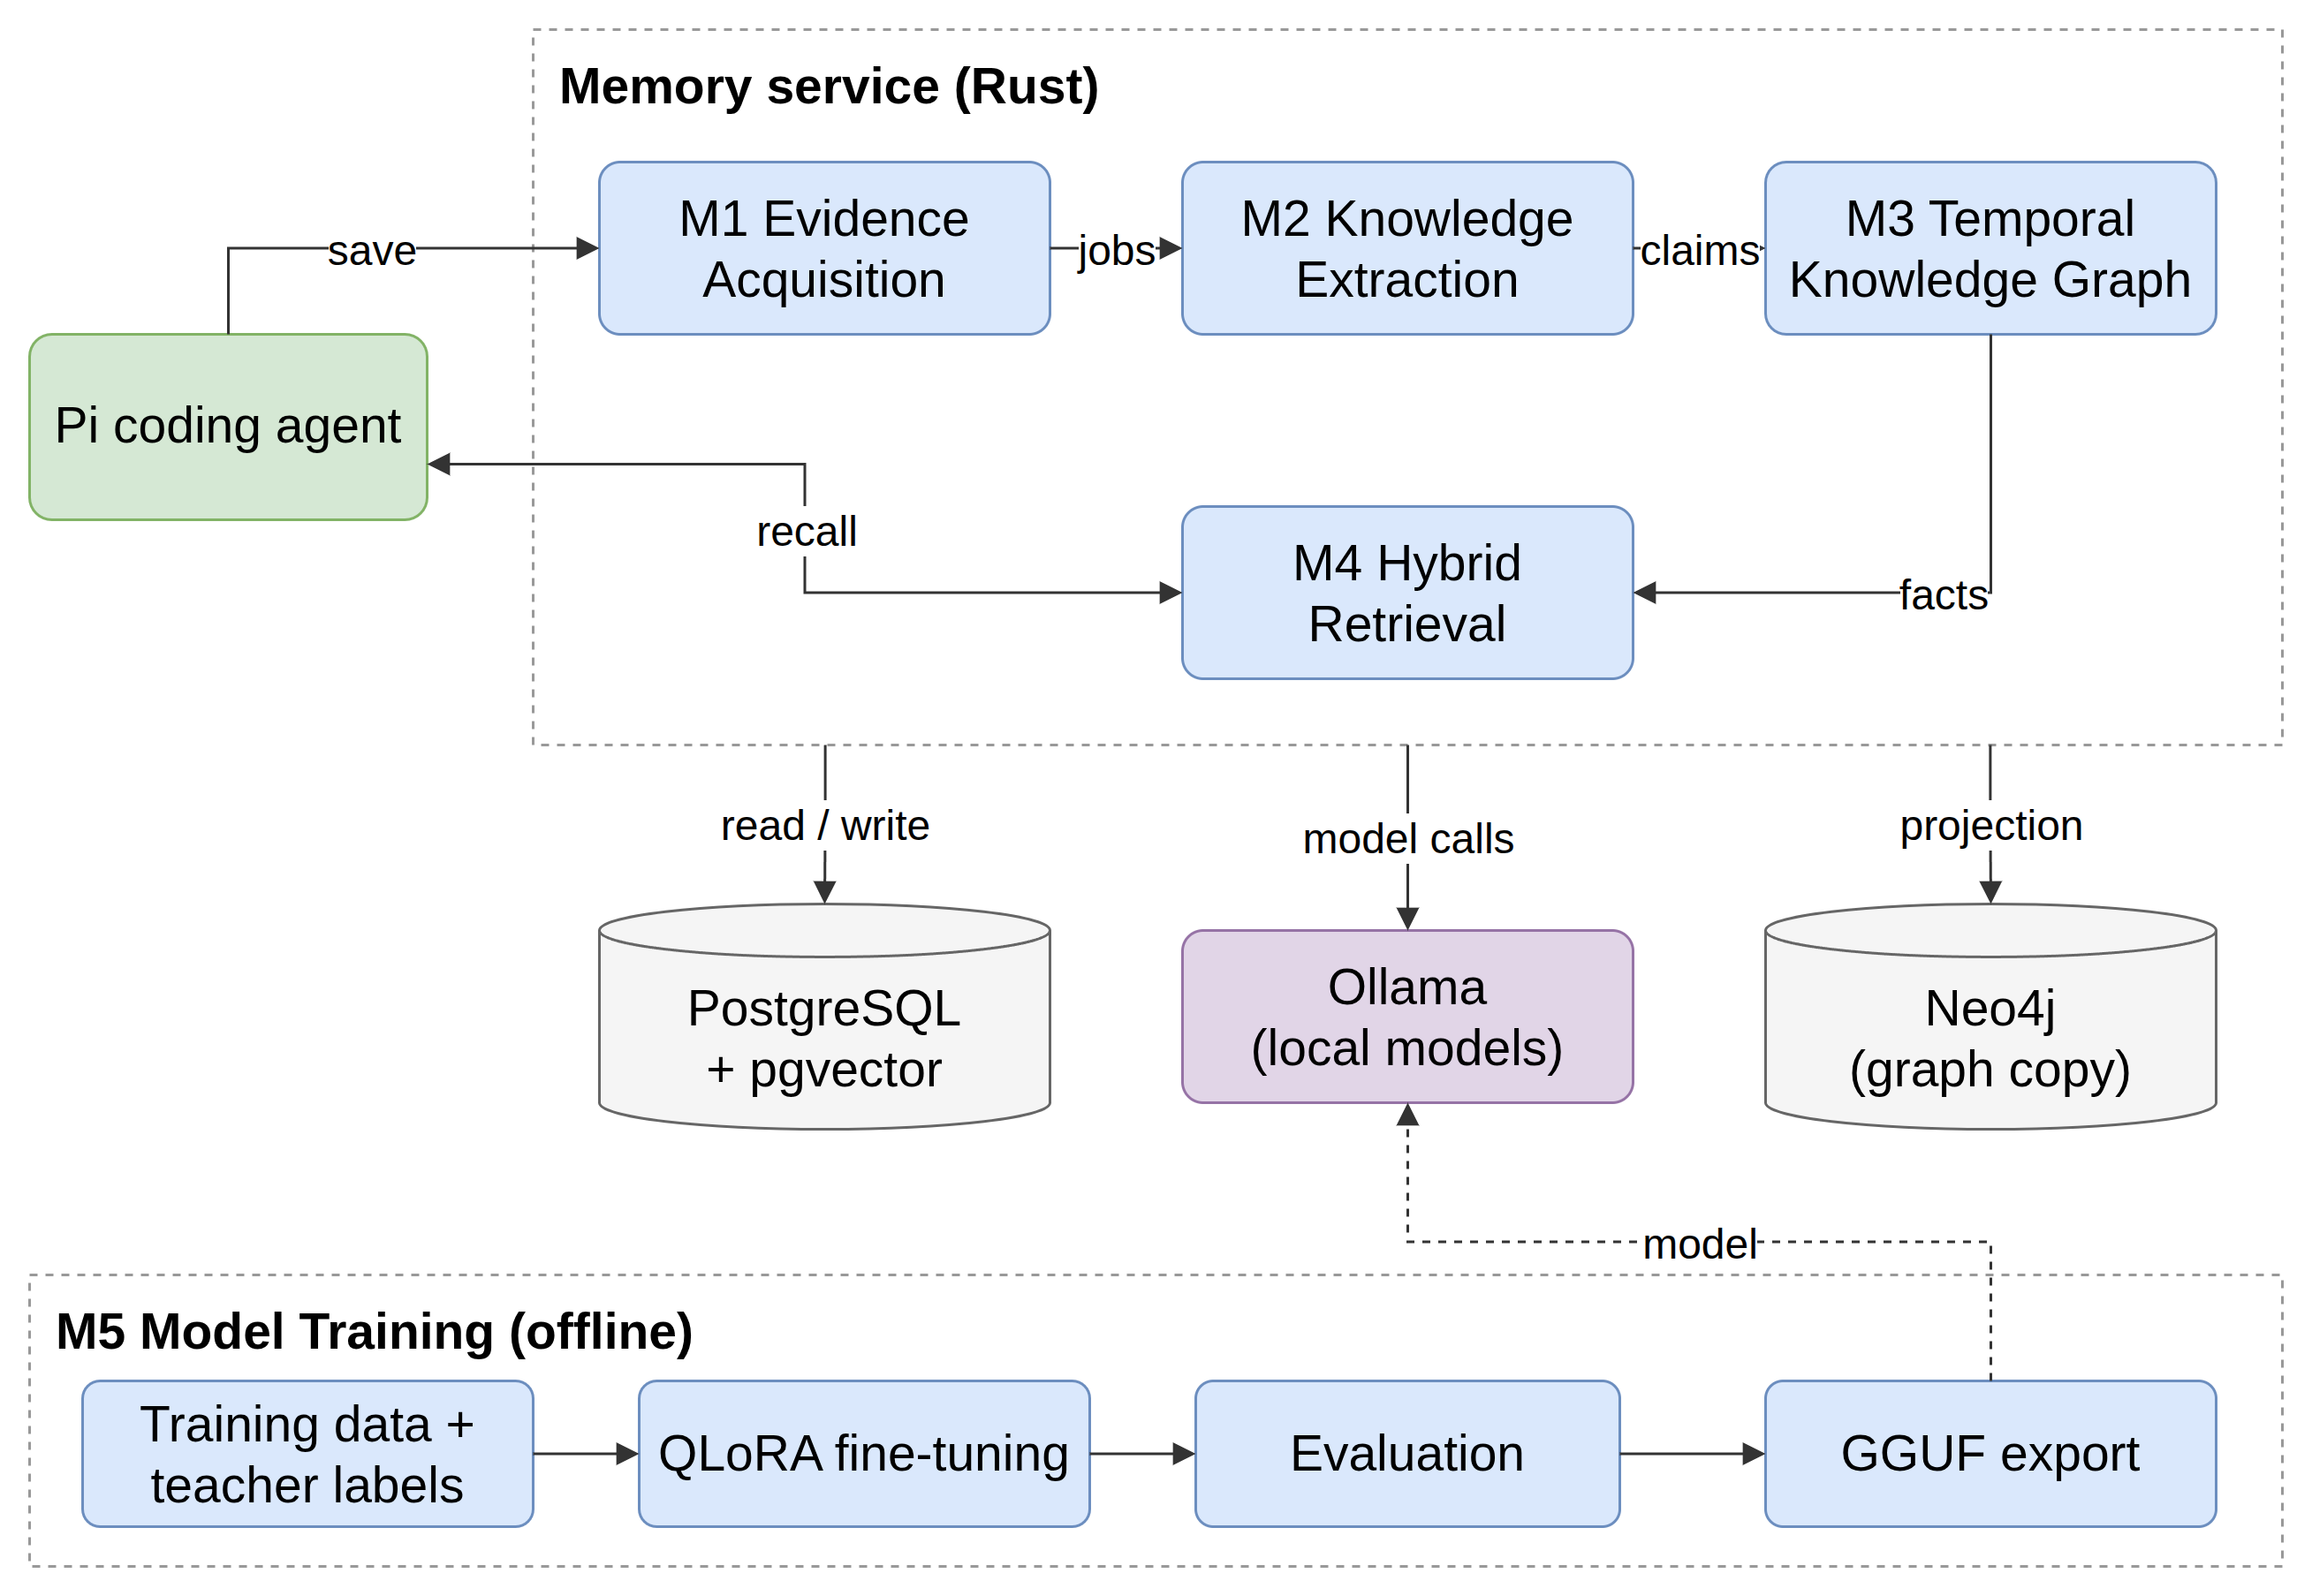
\includegraphics[width=\textwidth,height=0.5\textheight,keepaspectratio]{figures/fig3_1_architecture.png}
\caption{Overall system architecture}
\label{fig:architecture}
\end{figure}

\section{\uppercase{M1 Evidence Acquisition and Processing}}
M1 saves the evidence before anything else (Figure~\ref{fig:m1}). For Maya, the 10 October
conversation arrives as a retain request with namespace \code{user:maya}, session S2 and the
two events E3 (her message) and E4 (the agent's reply).

\begin{figure}[htbp]
\centering
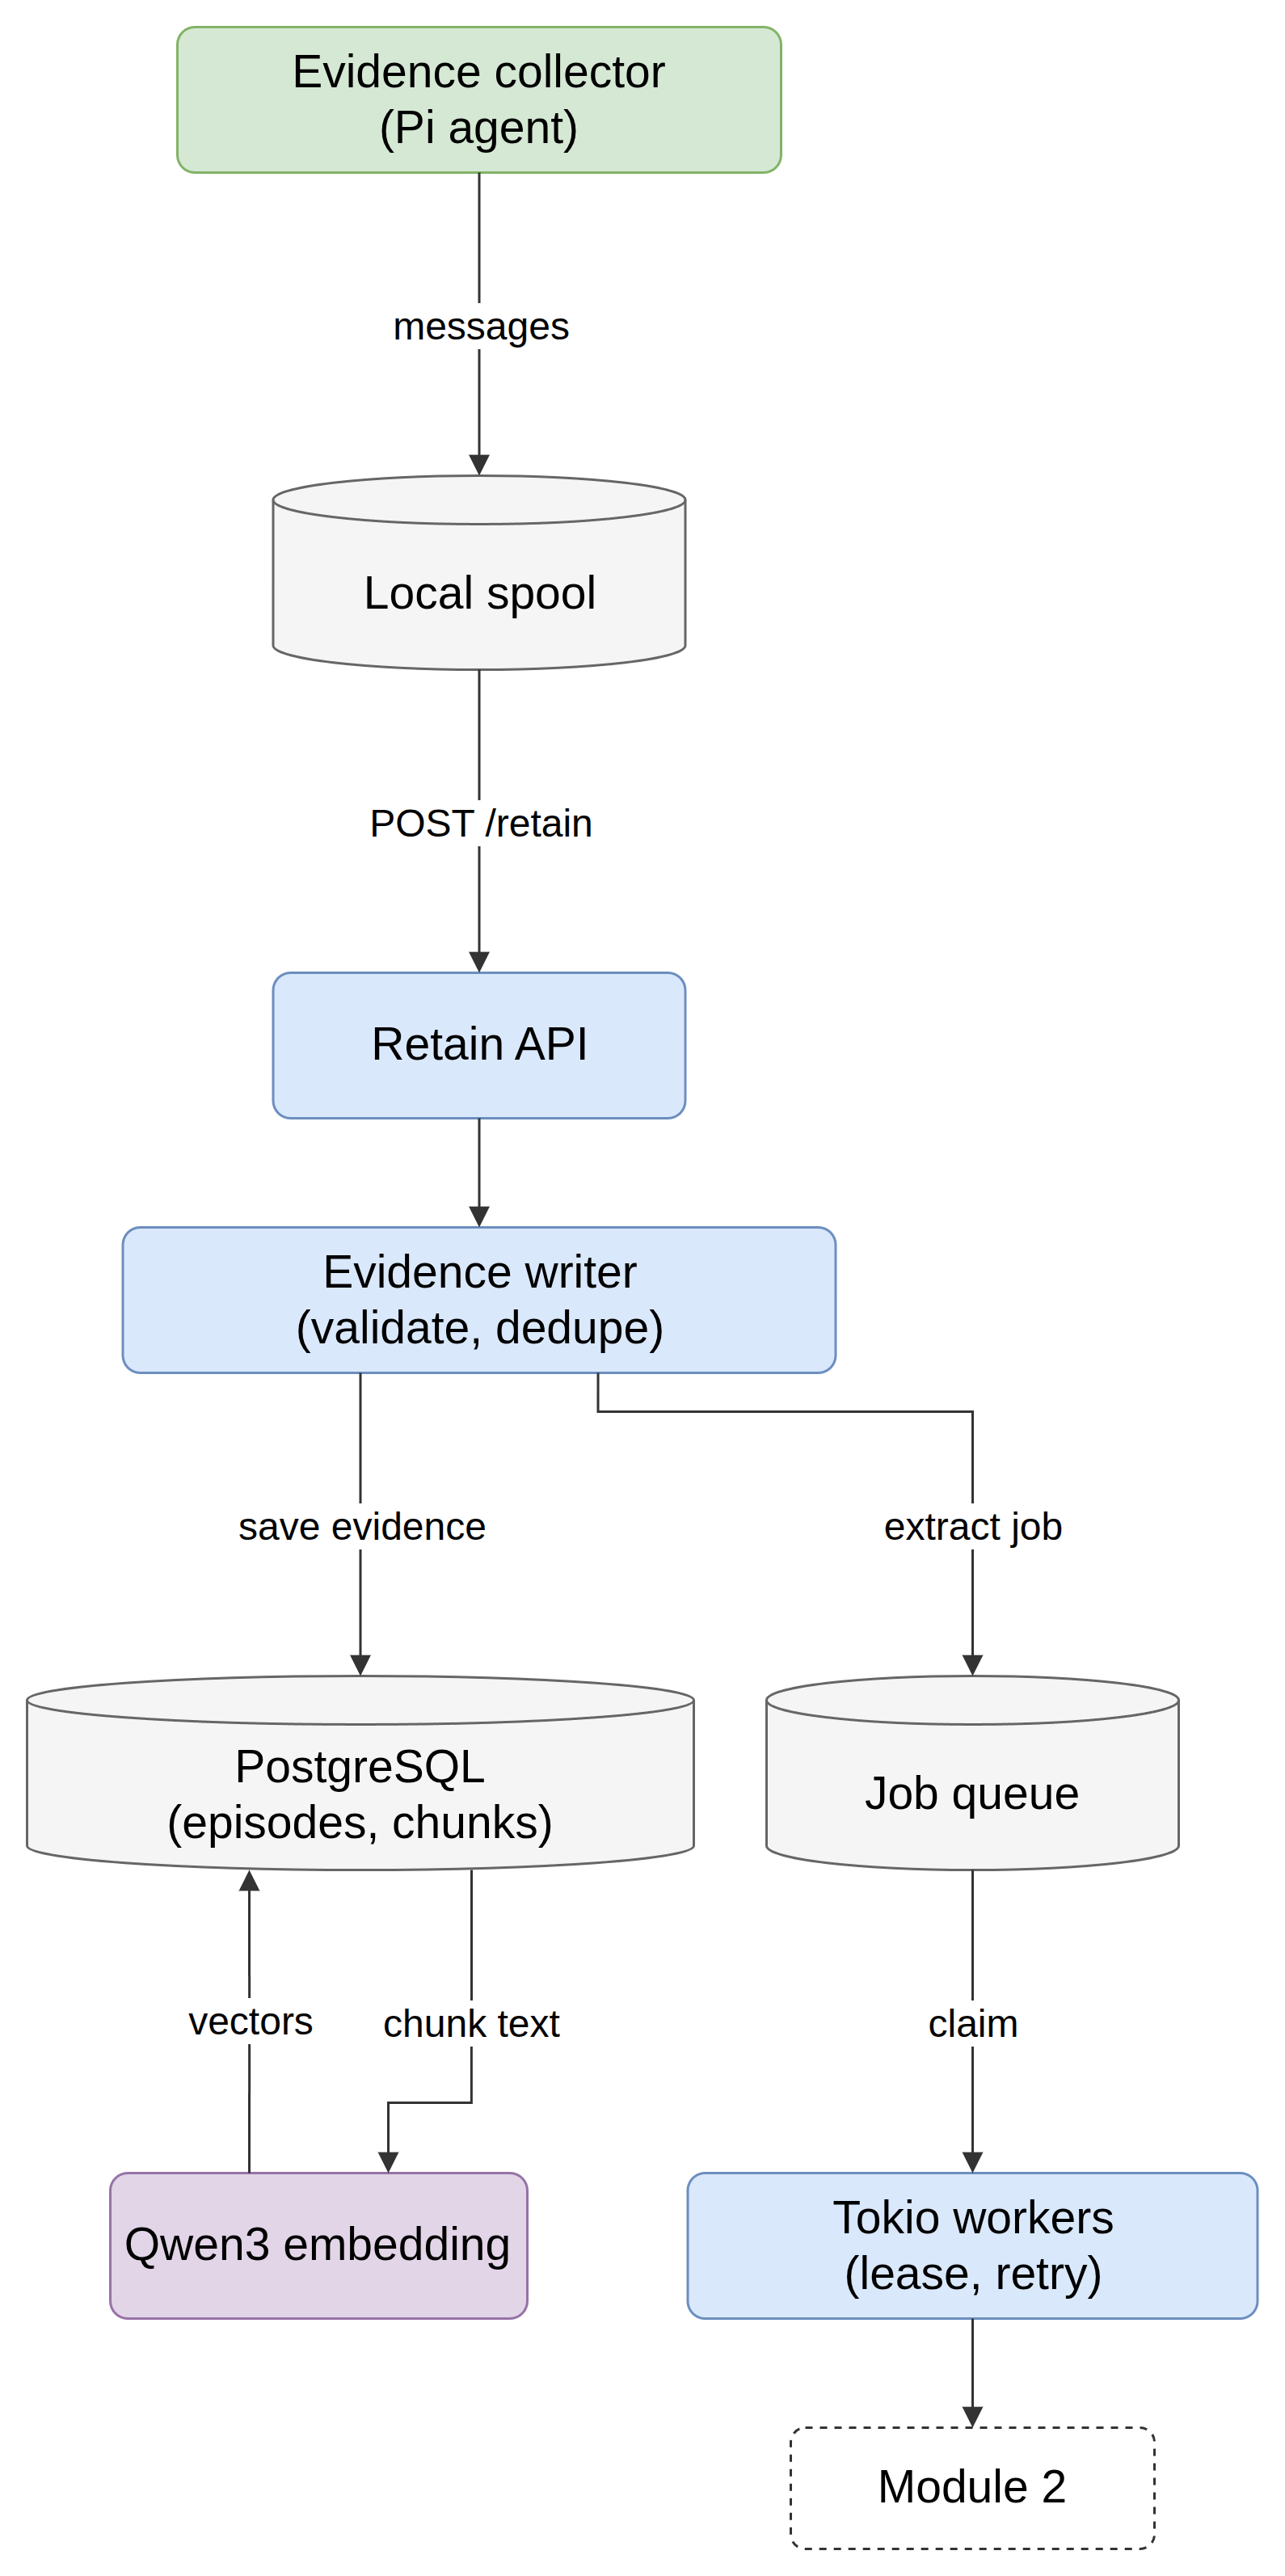
\includegraphics[width=\textwidth,height=0.5\textheight,keepaspectratio]{figures/fig3_2_module1.png}
\caption{Module 1: Evidence Acquisition and Processing}
\label{fig:m1}
\end{figure}

The evidence collector inside Pi gathers the role, text and timestamp of each
message on the current branch and forms a \code{RetainBatch}. This batch is first written
to a local spool of JSON files so nothing is lost if the service is down, and the spool
then sends it to \code{POST /api/v2/retain}. The writer checks the batch  (1 to 1,000 events). If the same key arrives again with the same SHA-256 hash it
just returns the existing IDs, so retries don't create duplicates; the same key with a
different payload gets HTTP 409. The episode, events and chunks are saved in one
transaction together with a pending extraction job in \code{memory\_jobs}. Each chunk is
also embedded into a 1,024-dimensional vector using \code{qwen3-embedding-cpu}.

Jobs are picked up by a pool of Tokio workers. A worker leases the namespace for 15
minutes (renewed every 30 s) and a job gets up to 5 tries with backoff up to 300 s. We run two workers locally (the default is four).
For Maya, M1 ends with episode P2 holding chunks C3 and C4, and job J2 pending. 

\section{\uppercase{M2 Knowledge Extraction and Consolidation}}
M2 has two stages, extraction and consolidation, and both call the same local model
\code{mem-extractor:general-v1} through Ollama (Figure~\ref{fig:m2}).  Outputs are cached in \code{model\_cache}.

\begin{figure}[htbp]
\centering
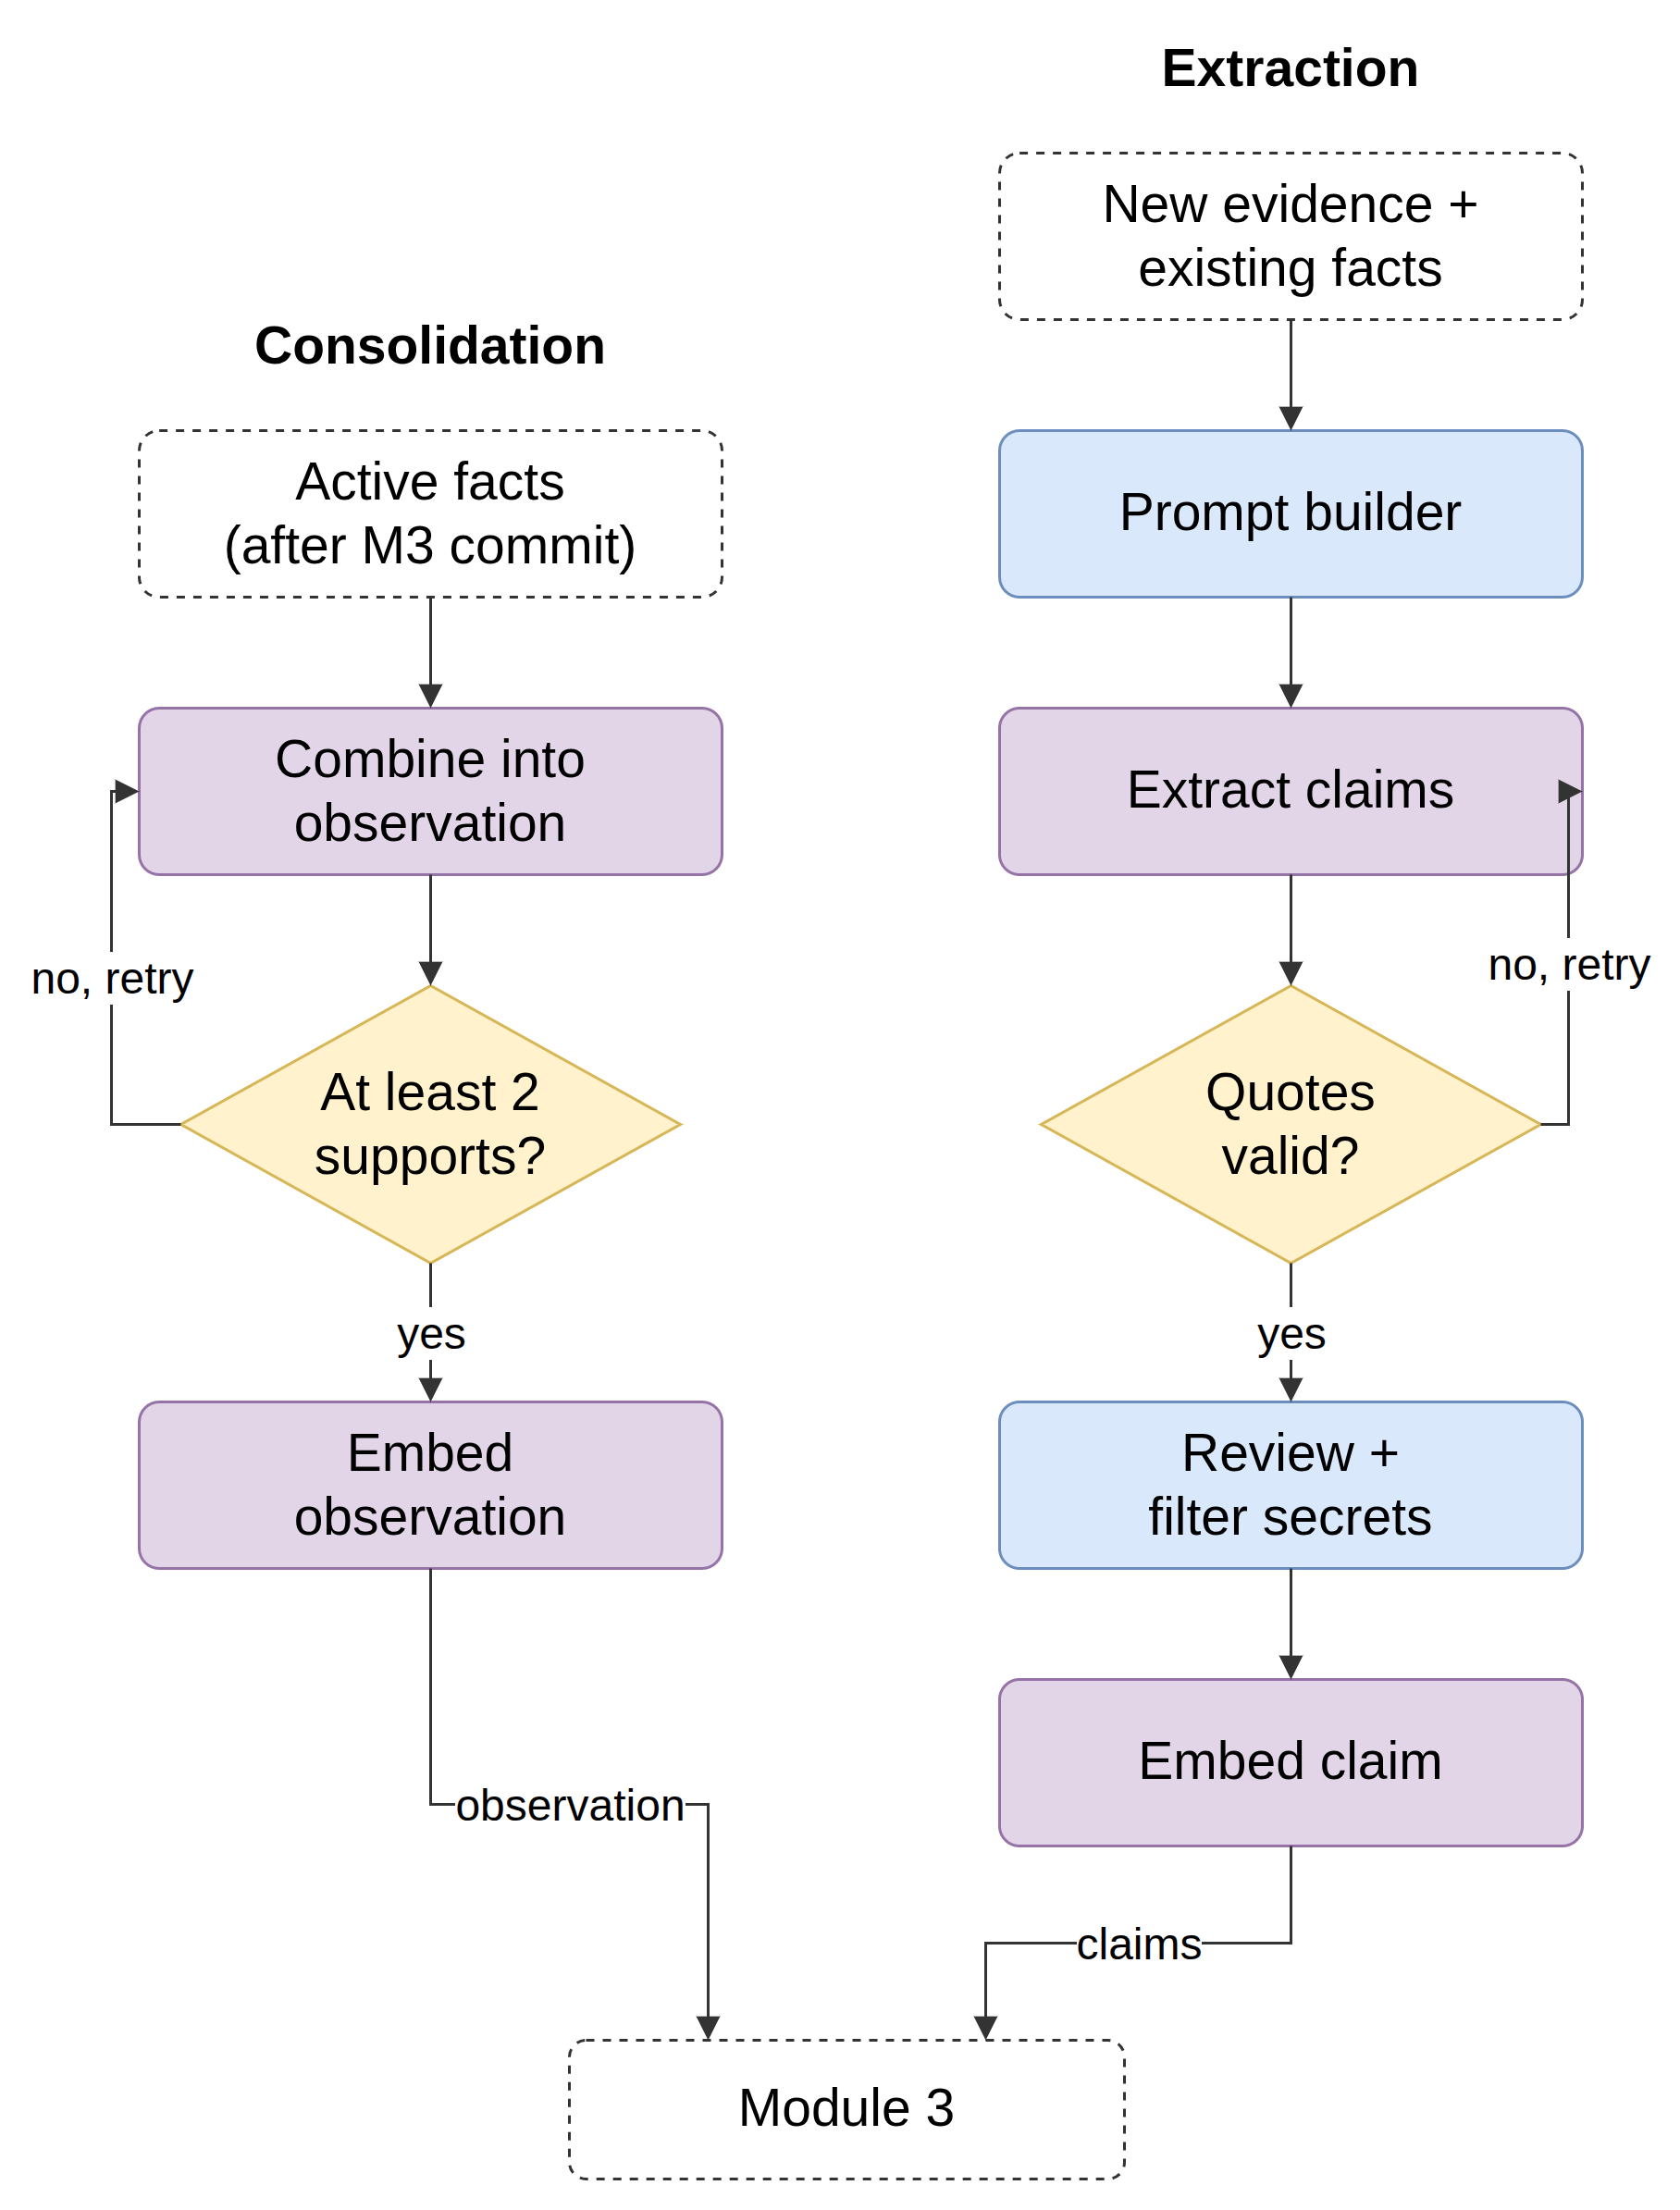
\includegraphics[width=\textwidth,height=0.5\textheight,keepaspectratio]{figures/fig3_3_module2.png}
\caption{Module 2: Knowledge Extraction and Consolidation}
\label{fig:m2}
\end{figure}

\textbf{Extraction.} The prompt builder fits the new evidence and the relevant existing
facts into the model's input (how existing facts are chosen is in Section~\ref{sec:alg-context}). For
Maya the existing fact ``Maya / Chennai'' is shown next to E3. The extractor returns
claims with exact quotes. Here it returns home city Bengaluru, single-valued and flagged as a
correction. The output is checked against the schema and each quote must appear
exactly in the source; if not, the model is asked again up to two times before the job
fails.  A review step confirms the correction, secrets are filtered out, and the claim ``Maya
lives in Bengaluru.'' goes to M3.

\textbf{Consolidation.} After M3 commits, M2 looks at the active facts of the changed
subject. If there are at least two, the model may combine them into one observation.
For Maya, the three work facts A1 (NovaTech), A2 (software engineer) and A3 (remote)
become ``Maya works remotely as a software engineer at NovaTech.''

\section{\uppercase{M3 Temporal Knowledge and Graph Management}}
M3 is the only module that writes the actual facts (assertions). Everything for one job
happens inside a single PostgreSQL transaction that holds a namespace lock and checks
the job's lease (Figure~\ref{fig:m3}).

\begin{figure}[htbp]
\centering
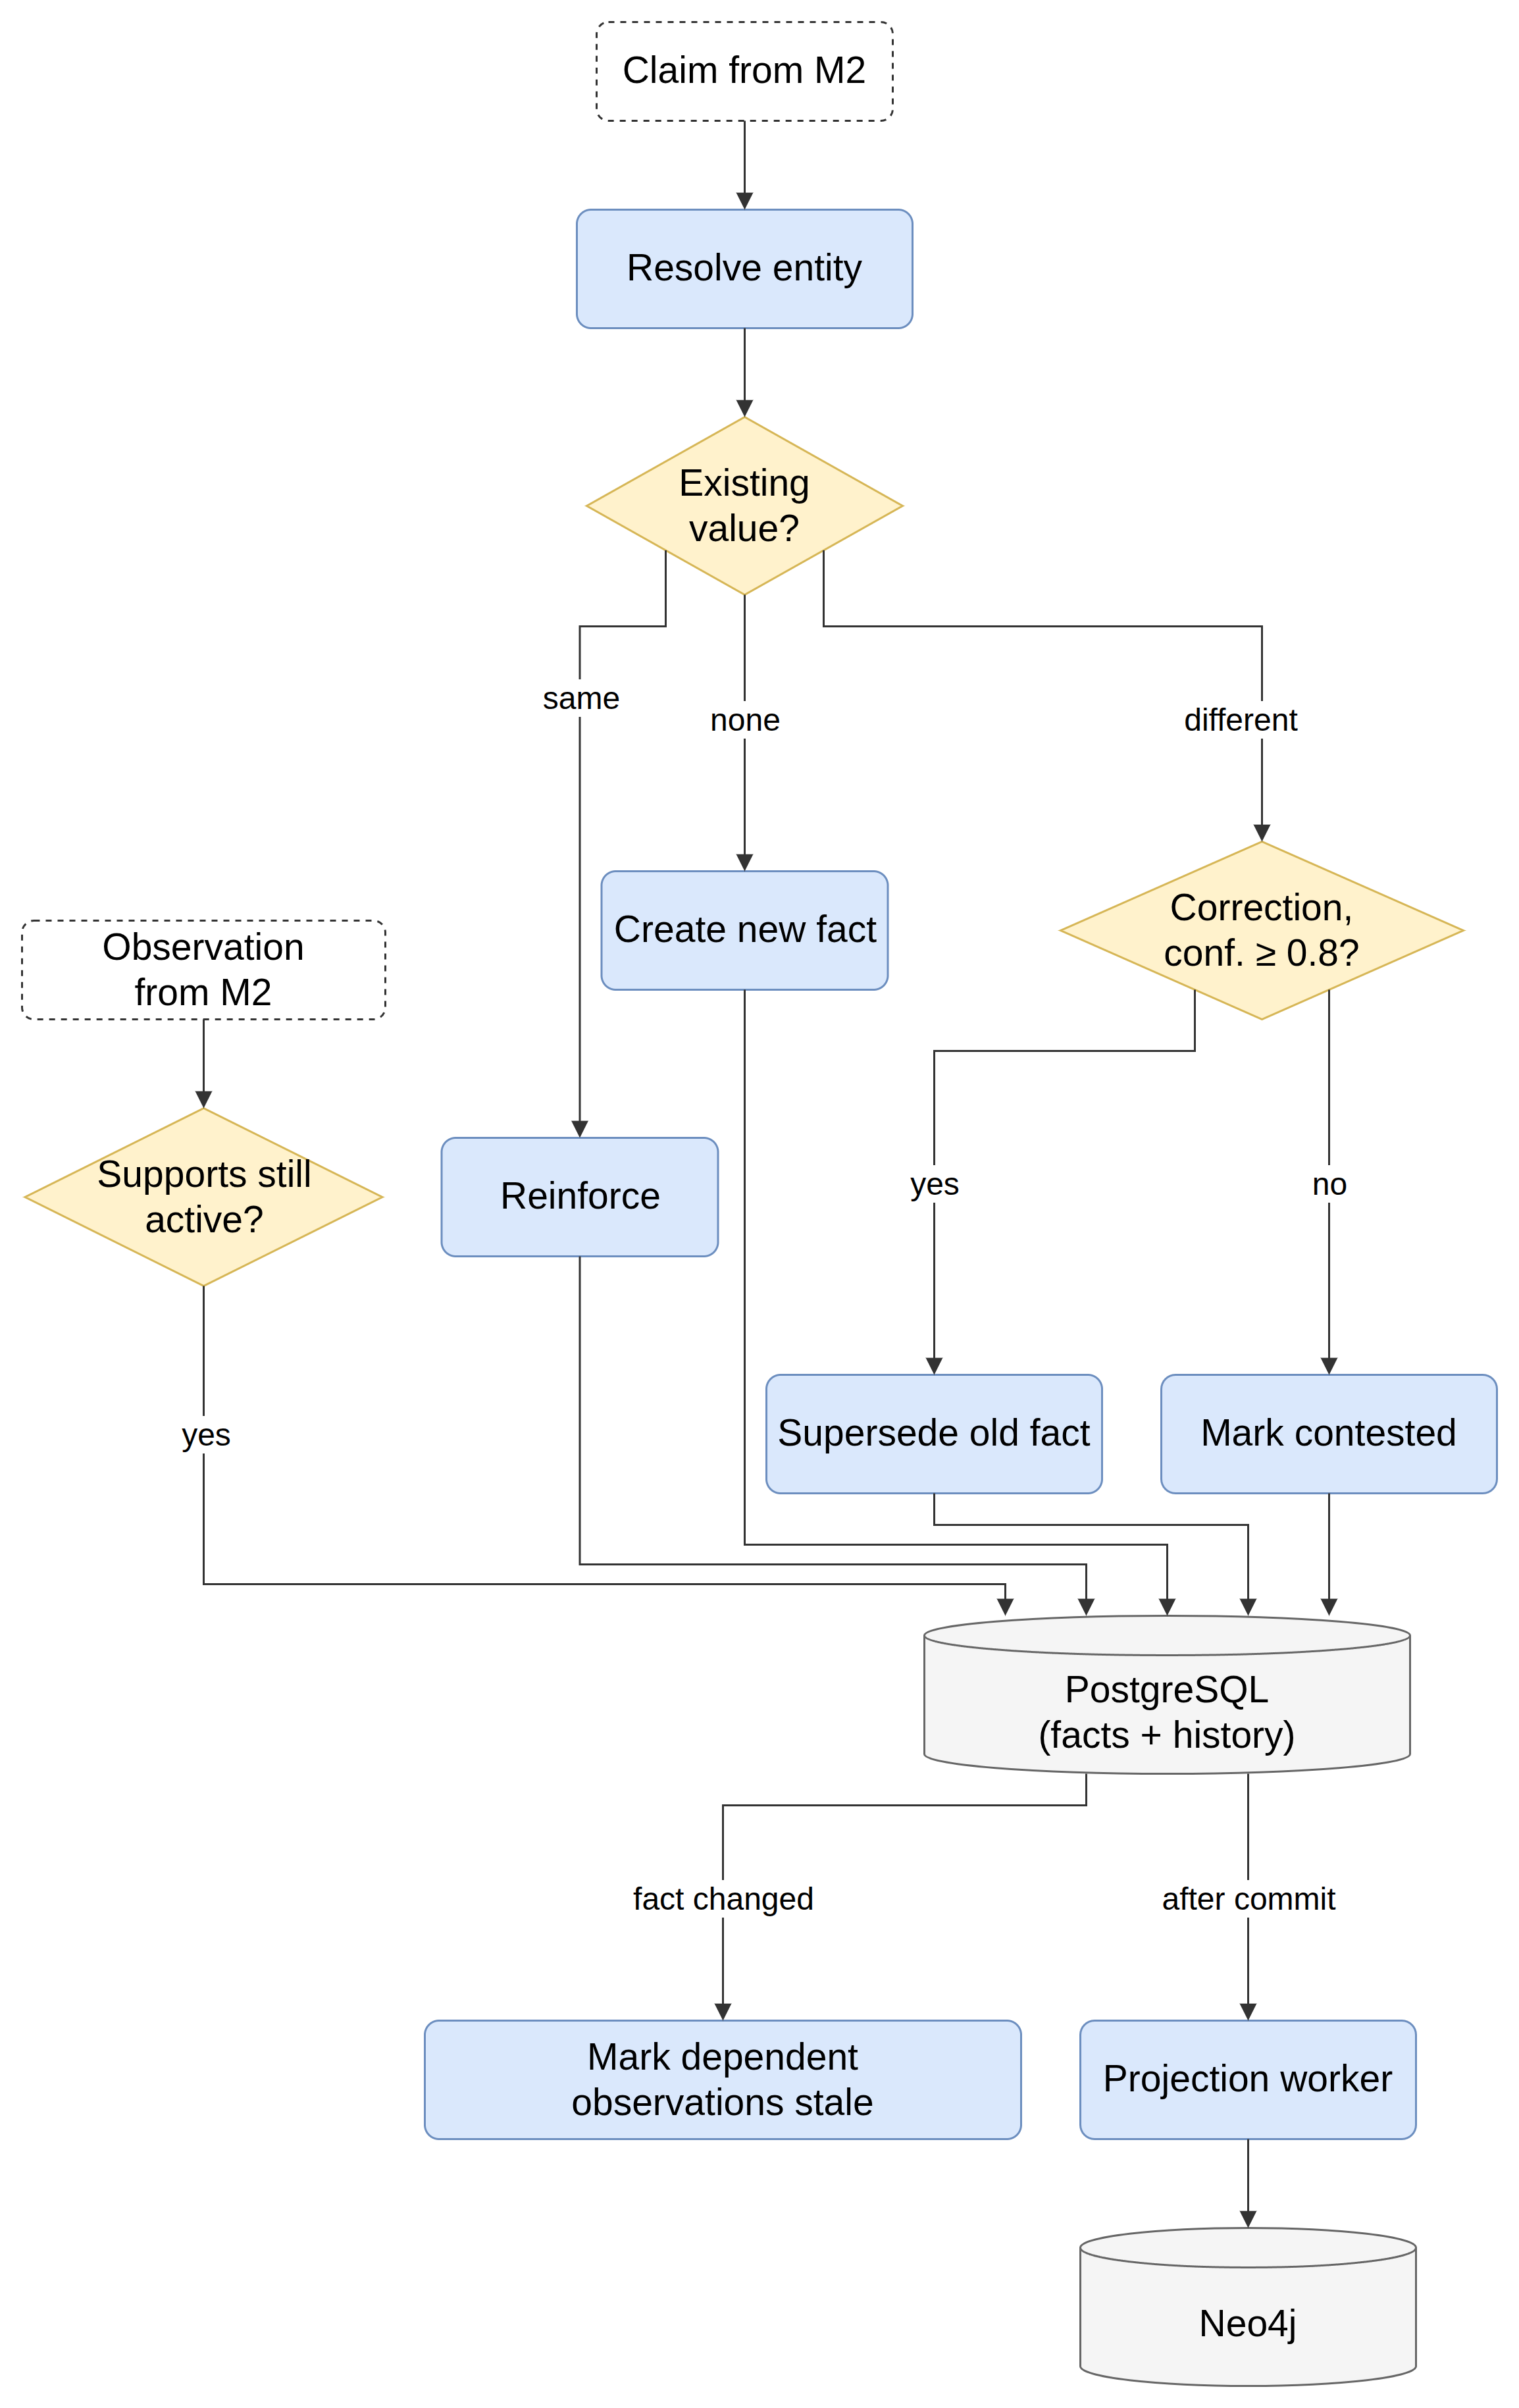
\includegraphics[width=\textwidth,height=0.55\textheight,keepaspectratio]{figures/fig3_4_module3.png}
\caption{Module 3: Temporal Knowledge and Graph Management}
\label{fig:m3}
\end{figure}

For a claim, M3 first resolves the entity (Maya, a person in \code{user:maya}). If the
same value already exists, it is just reinforced. If the slot is empty, a new active
assertion is made. The interesting case is a different value in a single-valued slot, like
Chennai to Bengaluru. If the claim is a reviewed correction with confidence at least
0.8, the old assertion is superseded and the new one becomes active; otherwise both are
marked contested. Maya's claim has confidence 0.95, so R1 Chennai becomes valid from
1 to 10 October and superseded, and R2 Bengaluru is active from 10 October, linked to
the E3 quote.

After the transaction commits, a projection worker copies the changed
assertion into Neo4j over HTTP \cite{neo4j2026http}.  These writes are revision-checked so an old revision can't overwrite a newer one.

\needspace{6\baselineskip}
\section{\uppercase{M4 Hybrid Retrieval and Grounded Reasoning}}
M4 answers recall requests (Figure~\ref{fig:m4}). On 13 October Pi sends E5 with namespace
\code{user:maya}, \code{top\_k} 10, a maximum distance of 0.45 and a 2,048 token budget.

\begin{figure}[H]
\centering
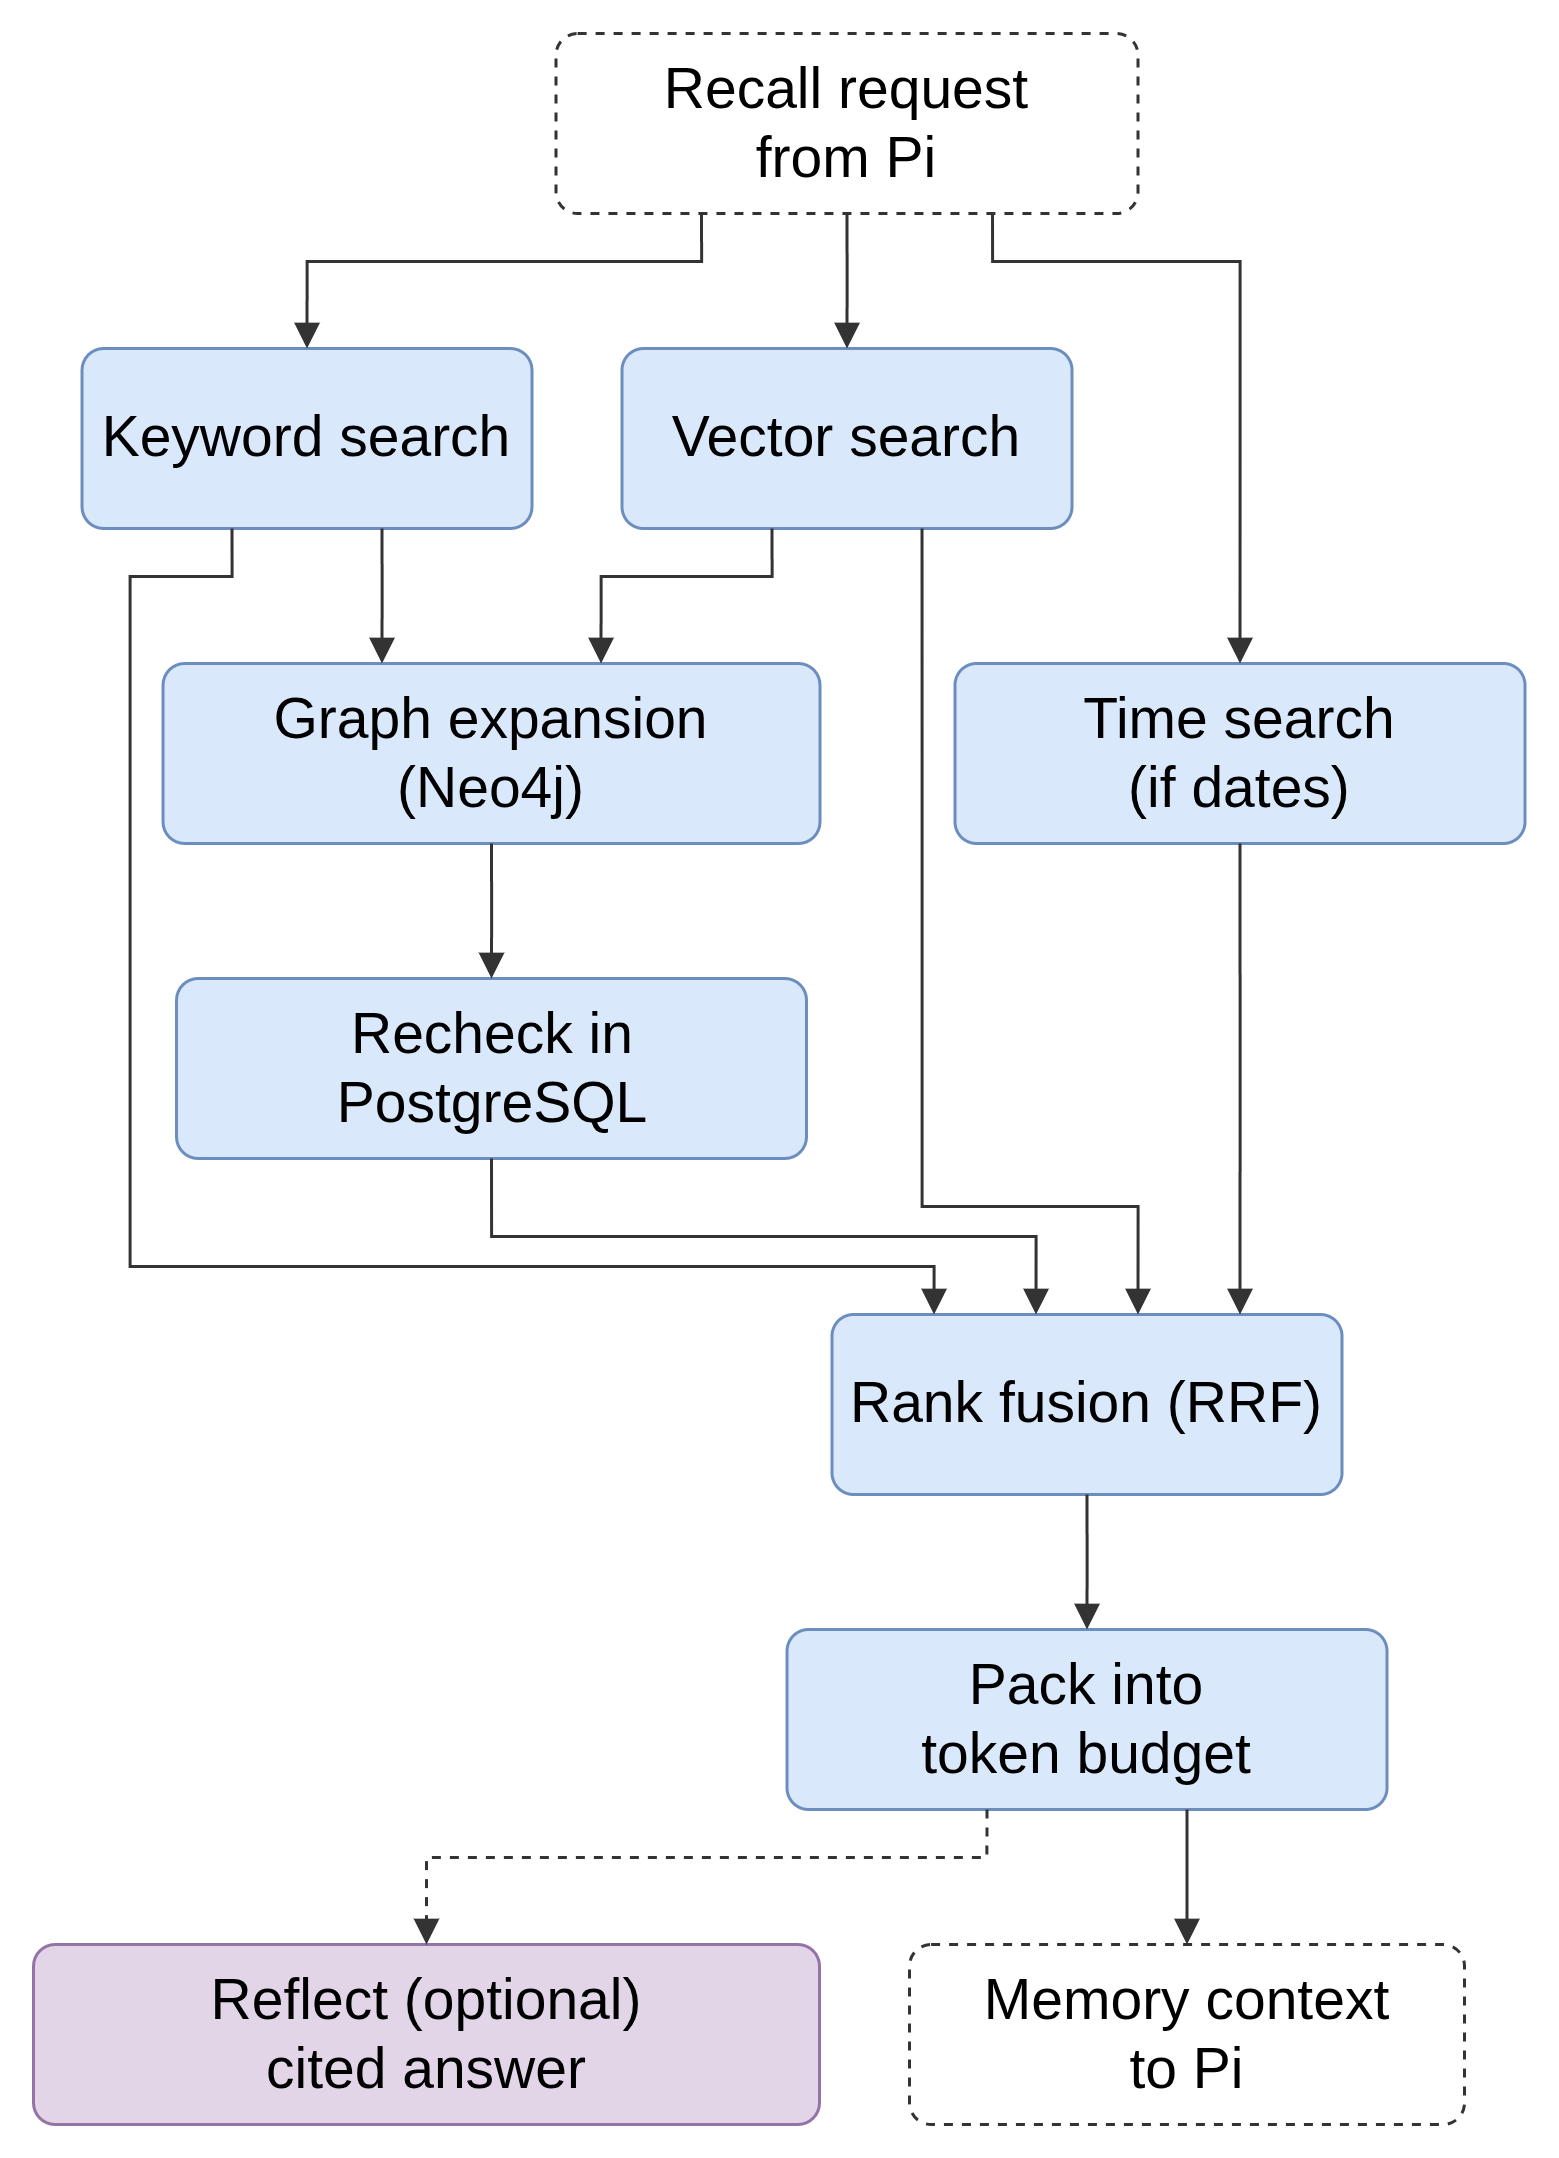
\includegraphics[width=\textwidth,height=0.45\textheight,keepaspectratio]{figures/fig3_5_module4.png}
\caption{Module 4: Hybrid Retrieval and Grounded Reasoning}
\label{fig:m4}
\end{figure}

The query goes to keyword, vector and (if there's a date window) time-based search,
the top results seed a Neo4j expansion, and the lists are merged with Reciprocal Rank
Fusion and packed into the budget with up to three quotes per hit. There is also an
optional reflect endpoint that writes a cited answer. All of this is in Chapter~\ref{ch:impl}.

\section{\uppercase{M5 Model Training and Evaluation}}
M5 runs offline and produces the worker model used by M2 and M4 (Figure~\ref{fig:m5}).

\begin{figure}[H]
\centering
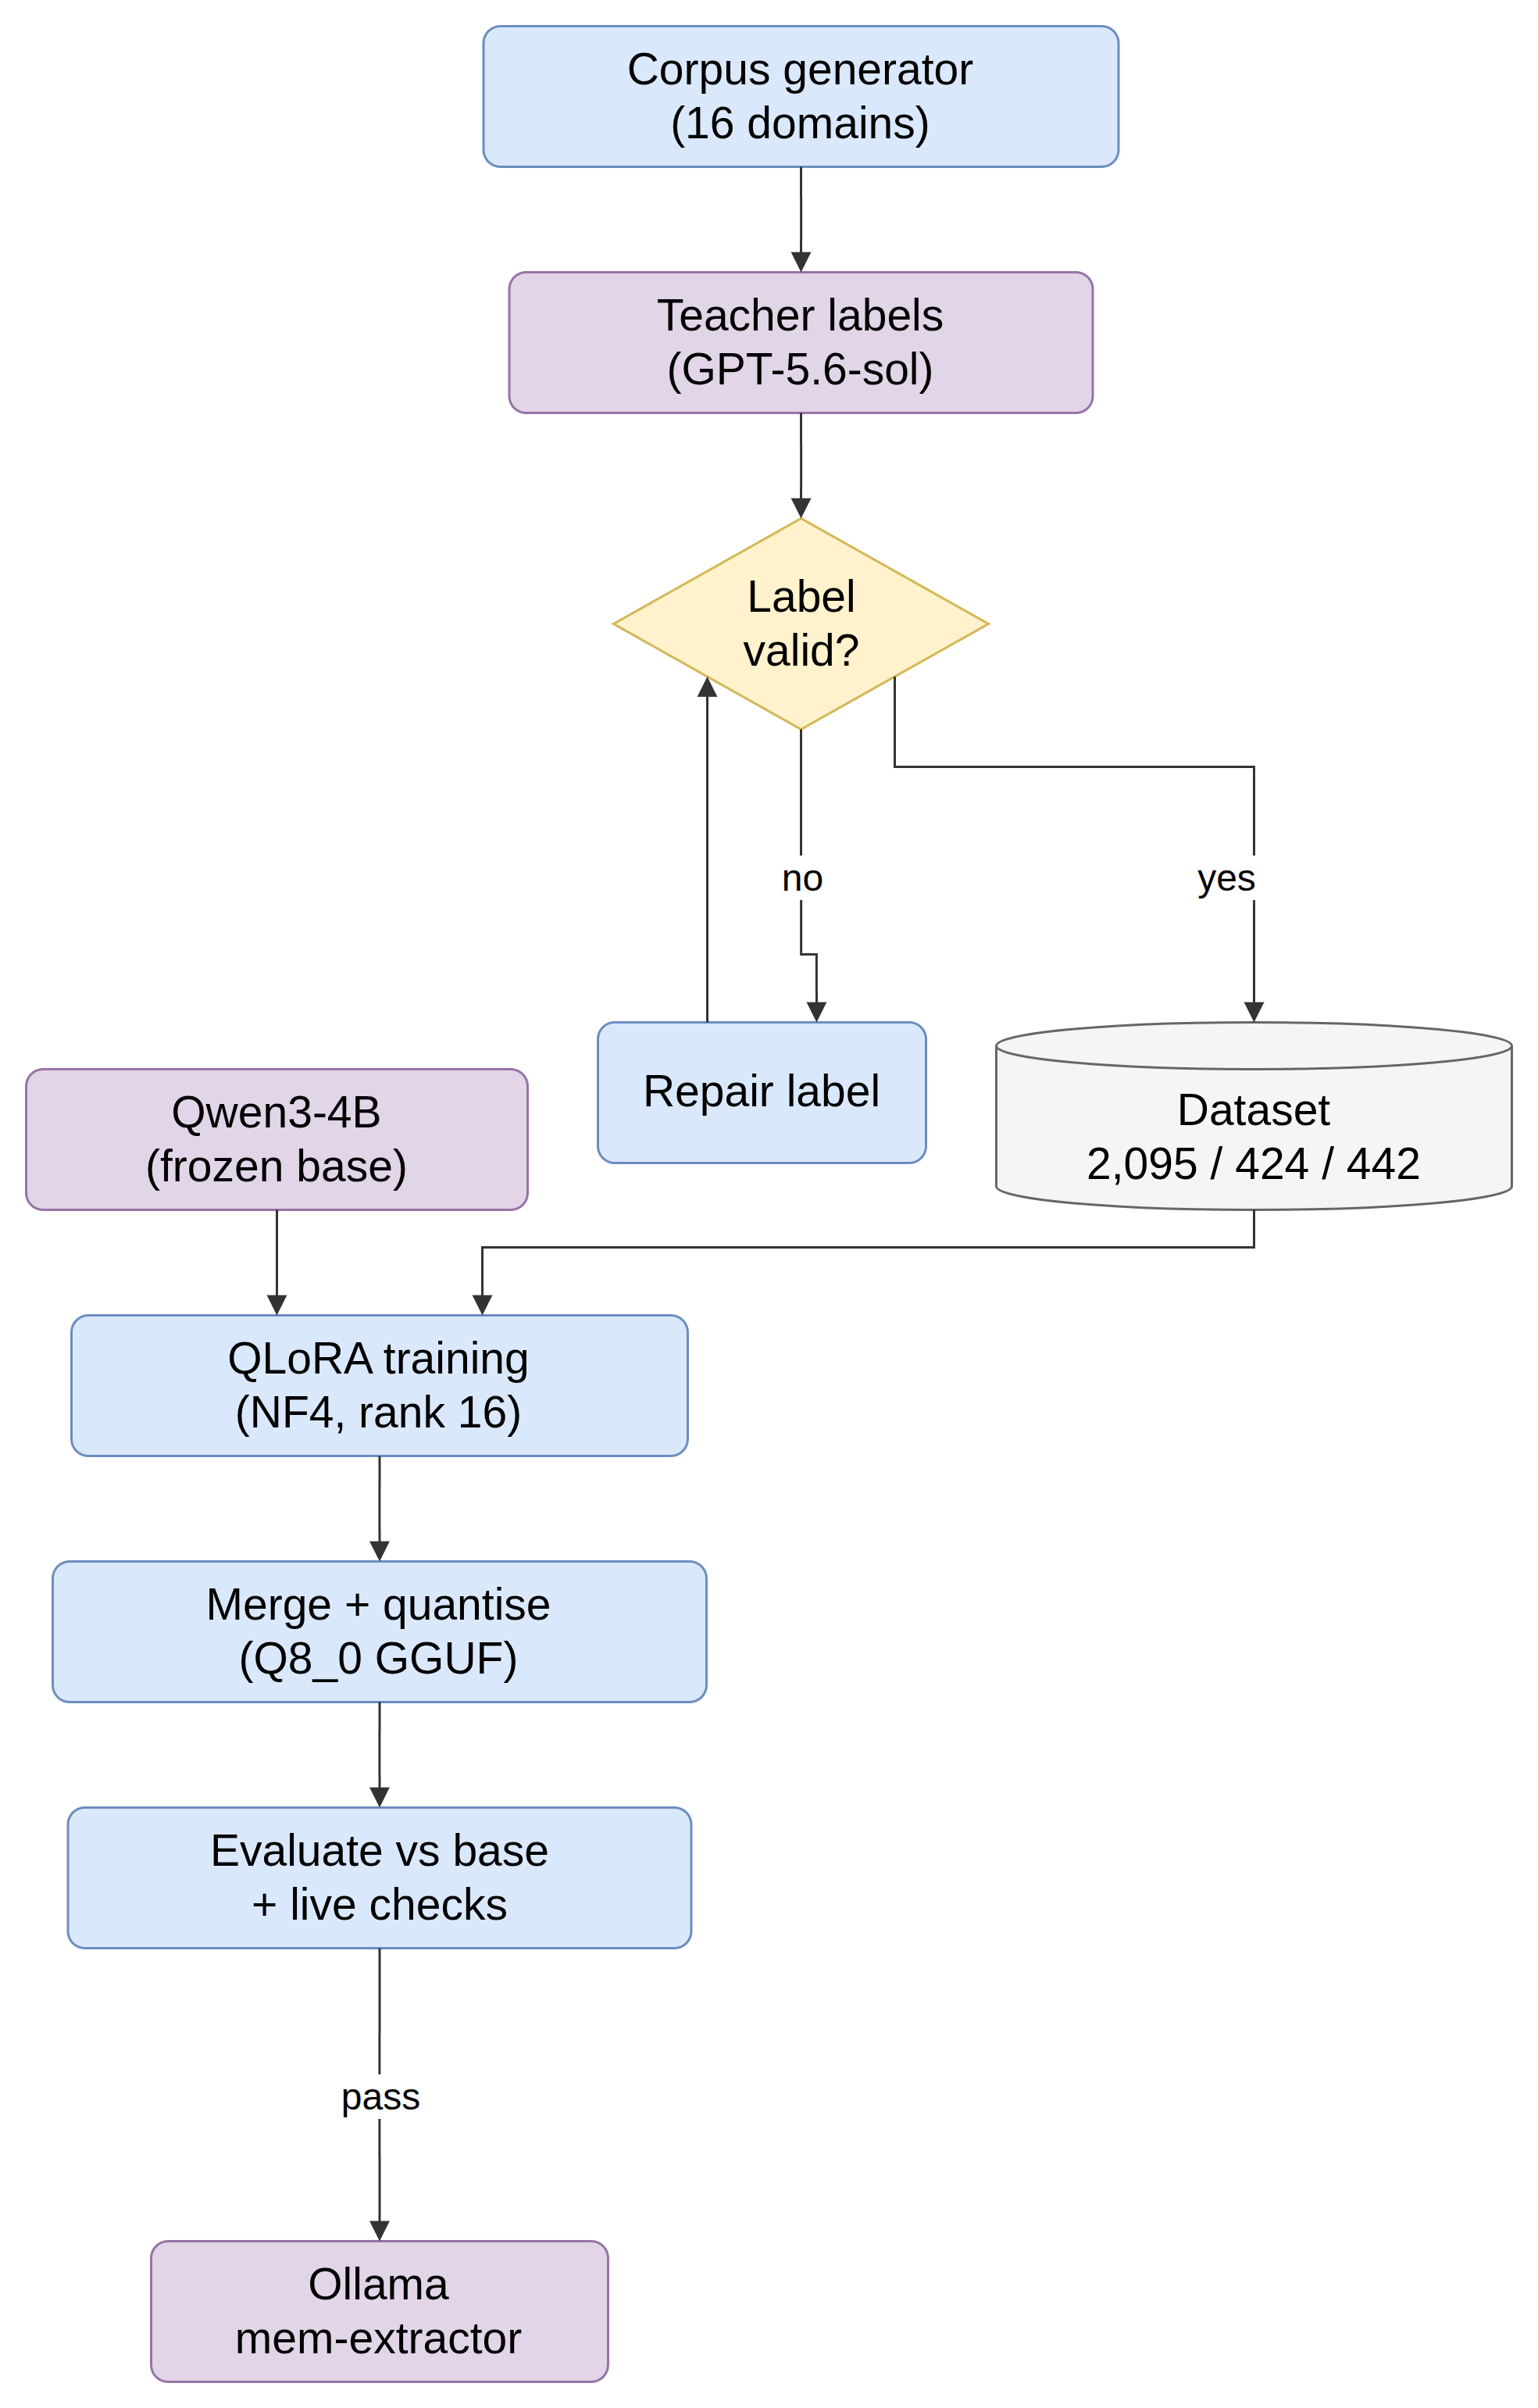
\includegraphics[width=\textwidth,height=0.4\textheight,keepaspectratio]{figures/fig3_6_module5.png}
\caption{Module 5: Model Training and Evaluation}
\label{fig:m5}
\end{figure}

A corpus generator makes short episodes across 16 domains (the Maya episode is one
of them) and a teacher model (GPT-5.6-sol) labels each one.  Checked labels form the dataset, and the
model is trained with QLoRA, evaluated and imported into Ollama (details in Chapter~\ref{ch:results}). 

So when Maya asks E5, Pi answers ``You now live in Bengaluru, following your move on
10 October 2026. Before that, you lived in Chennai. You work remotely as a software
engineer at NovaTech.''
